\begin{figure}[H]
\centering
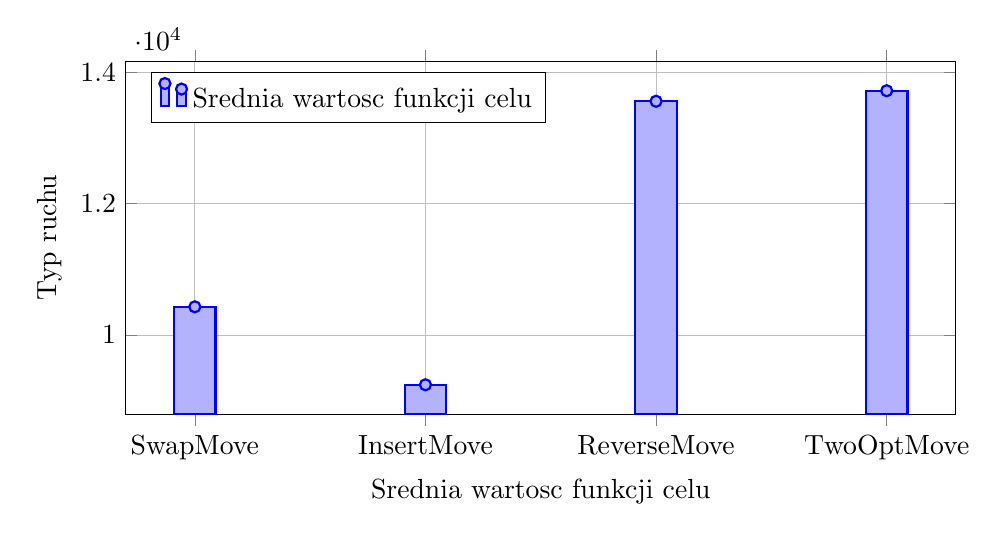
\begin{tikzpicture}
\begin{axis}[
xlabel = {Srednia wartosc funkcji celu},
ylabel = {Typ ruchu},
legend pos = north west,
grid = both,
width=1\linewidth,
height=0.5\linewidth,
ybar,
bar width=15pt,
symbolic x coords={SwapMove,InsertMove,ReverseMove,TwoOptMove,},
xtick=data
]
\addplot + [mark = *, thick] coordinates
    {
(SwapMove,10430.0)(InsertMove,9243.777777777777)(ReverseMove,13557.111111111111)(TwoOptMove,13717.388888888889)};
\addlegendentry
{Srednia wartosc funkcji celu}
\end{axis}
\end{tikzpicture}
\caption
{Srednia wartosc funkcji celu w zaleznosci od typu ruchu dla wszystkich instancji}
\label{fig:mean_goals_per_move_type_all_instances}
\end{figure}
